\chapter{Integrated Cases Across the Volumes}\label{v0ch:29}
\begin{chaptersummary}
The preceding chapters separated discrete operators, algebraic algorithms, and execution costs. Reproducible experiments now reconnect them: first verify the model, errors, and constraints, then record solution and data-movement costs. Comparing total time for a common problem and target error turns kernel analysis into an integrated computational decision.
\end{chaptersummary}
\learninggoals{Create consistent experiment records; complete Maxwell and high-order transport cases; distinguish kernel benchmarks, complete solves, and cross-model comparisons.}
\paragraph{Core Question}How can we establish that a faster implementation still solves the same problem?

\section{Krylov and AMG: From Poisson to Preconditioning}
Start with Volume I's two-dimensional Dirichlet Poisson discretization. Manufacture algebraic data to check direct, CG, and preconditioned true residuals; then use a continuous exact solution to assess discretization error. Record unknowns, $\nnz$, ordering, fill, setup, iterations, time, and error.
Use the algebraically manufactured right-hand side $\bm b=A\bm x_*$ to check the linear solver, then a continuous analytic solution to test PDE convergence. The code records these error levels separately. Multiple right-hand sides reuse the same factors to expose setup amortization, while the two-level AMG example verifies coarse-space correction.
Separate Krylov SpMV, preconditioning, dot products, and orthogonalization. Record AMG smoothing, restriction, coarse solve, and interpolation by level. At small sizes, fewer iterations may not offset setup and Python overhead; at large sizes, coarse communication and reductions can change the comparison. Serial teaching hierarchies do not measure distributed AMG scaling.
\section{Complete Maxwell Evolution}
On the periodic unit cube with vacuum $c=1$, use the right-going transverse wave
\[
 E_y(x,t)=\sin(2\pi(x-t)),\qquad B_z(x,t)=\sin(2\pi(x-t)).
\]
All other components vanish. Initialize the magnetic field at its own spatial locations and $t=-\Delta t/2$, choosing
$\Delta t\le\nu h$, $\nu<1/\sqrt3$, and adjusting the step to reach the same $T$ exactly. Compare $L^2$ error, phase, steps, and time on two grids. Half-time initial data must not be treated as full-time values.
The CPU code also computes curls of random edge fields, checking divergence and monitoring $\diverg_h B$ and modified energy. The source-free electric-divergence test represents zero charge; sources require compatible current and continuity updates.
\begin{figure}[htbp]\centering
\IfFileExists{Vol0_Linear_Algebra_HPC/figures/convergence.pdf}{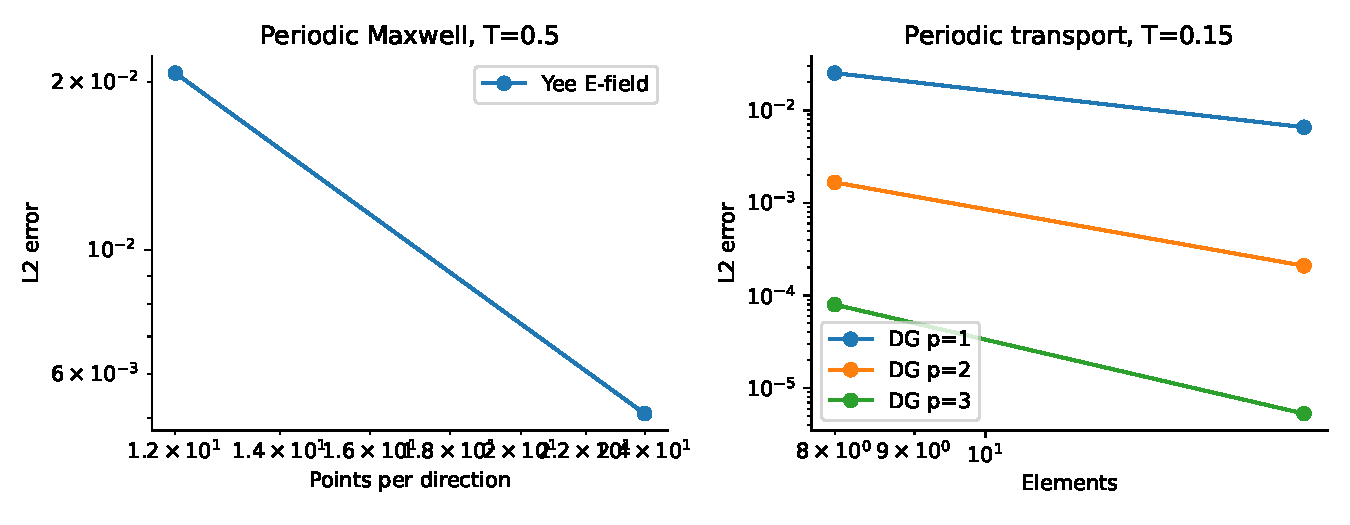
\includegraphics[width=.88\textwidth]{Vol0_Linear_Algebra_HPC/figures/convergence.pdf}}{}
\caption{Measured CPU convergence data for Yee transverse waves and periodic transport. Error definitions and parameters accompany the records.}
\end{figure}
GPU execution preserves SoA, phase order, and initial data. MPI exchanges required fields per phase before interior/boundary work. The CUDA full-field program provides a device path; the MPI solver includes phase halos and global constraints. The appendix and data record execution scope; cross-node and multi-GPU coupling can then be measured under the same error and constraint conventions.
\section{Complete High-Order DG and the FR Interface}
For $u_t+u_x=0$ with periodic $u(x,0)=\sin(2\pi x)$, use elementwise Legendre modes
$u_h=\sum_{m=0}^{p}\widehat u_mP_m(\xi)$. The weak form is
\[
 \frac h2 M\dot{\widehat{\bm u}}
 =S\widehat{\bm u}-\bm\phi(1)\widehat f_R
                         +\bm\phi(-1)\widehat f_L,\quad
 M_{mm}=\frac2{2m+1},\quad S_{m\ell}=\int_{-1}^{1}P'_mP_\ell.
\]
For positive speed, upwinding takes the left trace. Volume terms, face fluxes, and diagonal mass inversion are directly implementable. RK4 with conservative steps compares $p=1,2,3$ and element counts in error, unknowns, steps, and time.
At the two $p=1$ Lobatto endpoints, the FR test uses
$g_L=(P_2-P_1)/2$, $g_R=(P_2+P_1)/2$
Construct derivative corrections and verify equivalence with nodal DG under the same exact-mass and quadrature conventions. For other correction functions, compare their lifting and volume operators directly. Three-dimensional tensor derivatives are also checked against dense Kronecker application to verify sum factorization.
MPI partitions elements, exchanges upwind traces at every RK stage, and retains local mass inversion. GPU optimization can batch same-order elements, reuse derivative matrices, and separate volume/face work. Increasing order raises register demand and volume-to-face ratio. Executed GPU checks currently cover Yee and layout; a complete DG GPU port is a separate extension.
\conceptbridge{Why can higher kernel throughput accompany a slower complete DG run?}{High-order local work increases intensity but also changes stable steps, stages, and error. Local throughput becomes an end-to-end benefit only through the element and step counts required for target accuracy.}{Kernel reuse $\longrightarrow$ accuracy and stable step $\longrightarrow$ cost to physical final time.}
\section{Access Comparisons: FDM, FVM, FEM, and LBM}
First-order upwind FVM solves the same periodic transport problem as DG, enabling error and total-time comparisons. Seven-point FDM, Yee, DG tensors, LBM streaming and collision, and CSR/GEMM expose different access patterns. Cross-model update rates describe implementation signatures; method selection uses a common physical problem and target error.
FEM checks assembled against local matrix-free actions. FVM/DG checks shared-flux conservation; LBM checks periodic mass. Accept correctness before timing.
\subsection{Regular and Staggered Stencils}
Seven-point FDM outputs one scalar field per application; Yee updates six staggered components in two phases. Both support contiguous indexing and halos, but equal site counts imply neither equal unknowns nor equal physics. Distinguish the 8-FLOP Laplacian, 42-FLOP difference-based Yee, and 30-FLOP fused Yee, stating traffic assumptions.
\subsection{Adjacency, Irregular Access, and Geometry}
The FVM case renumbers nonuniform periodic cells, gathers states through left/right face indices, computes fluxes, and accumulates residuals. Verify permutation equivalence and zero volume-weighted residual sum. This isolates numbering and gather/scatter. General unstructured meshes additionally require normals, areas, reconstruction neighborhoods, and graph partitioning. MPI exchanges follow partition-crossing faces, not a presumed fixed array-neighbor pattern.
\subsection{Local Matrices and Population Layout}
One-dimensional P1 FEM compares CSR with elementwise difference accumulation under identical boundary elimination. LBM separately times streaming, collision, and complete steps. Streaming tests check push/pull and AoS/SoA equality; periodic BGK checks mass. Collision live variables and boundary branches also influence GPU occupancy, which a CPU layout test alone cannot predict.
\paragraph{The Eight Case Interfaces}
FDM--Yee stencils, FVM adjacency, DG/FR volume/face structure, LBM streaming/collision, Krylov, AMG, complete Maxwell, and complete high-order DG cover eight performance interfaces. Code and appendices specify acceptance criteria and execution scopes.
\section{Common Acceptance and Selection}
\begin{center}\small
\begin{tabularx}{\textwidth}{lX}
\toprule Dimension&Required record\\\midrule
Physics/discretization&Equations, boundaries, initial data, $T$, mesh, order, unknowns\\
Accuracy&Space/time error, phase, true residual, conservation, constraints\\
Algorithmic work&Steps, stages, iterations, preconditioning, hierarchy complexity\\
Resources&Array/factor storage, modeled FLOPs/traffic, messages, reductions\\
Timing scope&Inclusion of setup, advance, transfer, communication, checks, output\\\bottomrule
\end{tabularx}
\end{center}
\costnote{Fixed-unknown comparisons analyze implementations; fixed-error comparisons select methods. Report both. Small CPU tests validate the workflow; large-scale optimization requires representative working sets, parallel scale, and counters.}
\coderef{run_all.py; run_accelerators.py; fdtd/yee.py; dg_fr/transport.py}
\aiexercise{Run the experiments and plot error against time and unknown count from JSON. Check that physics, final time, and error norm agree within each comparison.}{Choose an error threshold and search mesh, order, and time step jointly for Yee or DG, including setup, communication, and output in the budget.}
\studyroute{Cross-node benchmarks and engineering-scale complex boundaries are further experiments. The experiment guide supplies reproduction commands and timing conventions. References: \cite{yee,hesthaven,roofline}.}{verification versus validation; manufactured solution; error versus cost; constraint preservation; time to solution}
